\section{Lasso estimatoren} \label{sec:lasso_estimatoren}
\textit{Dette afsnit er skrevet udfra kapitel 2 i \citep{hastie}.}

\textit{The Least Absolute Shrinkage Selection Operator}, som forkortes lasso, blev introduceret i \citep{lasso}. 
Lasso finder løsningen til optimeringsproblemet
\begin{align}
\hat{\beta}^\text{lasso} = \argmin_{\beta} \cbr{\frac{1}{2n} \sum_{i=1}^n \del{y_i - \sum_{j=1}^p x_{ij} \beta_j}^2}, \ \text{underlagt at } \sum_{j=1}^p \vert \beta_j \vert \leq t, \label{eq:2.3}
\end{align} 
hvor vi bemærker, at betingelsen $\sum_{j=1}^p \vert \beta_j \vert \leq t$ kan skrives mere kompakt som en \(\ell_1\)-norm betingelse $\Vert \beta \Vert_1 \leq t$.
Værdi af \(t\) begrænser summen af de absolutte værdier af parameter estimaterne.
Den kontrollerer kompleksiteten af modellen. 
En lav værdi af \(t\) vil begrænse antallet af parametre, hvilket fører til en sparse model, som tilpasser data mindre præcis, mens en høj værdi af \(t\) betyder flere parametre og tillader dermed, at modellen tilpasser data meget præcis.
Værdien af \(t\) skal specificeres ved en ekstern procedure kaldet \textit{krydsvalidering}, som vil blive diskuteret i kapitel \ref{kap:statistisk_inferens}.

Lasso problemet kan omskrives til et Lagrange problem
\begin{align}
\hat{\beta}^\text{lasso} = \argmin_{\beta} \cbr{\frac{1}{2n} \Vert \y - \X \beta \Vert_2^2 + \lambda \Vert \beta \Vert_1}, \label{eq:2.5}
\end{align}
hvor $\lambda \geq 0$ er en såkaldt strafparameter, som også bestemmes udfra krydsvalidering. 
Der er en en-til-en korrespondance mellem det betingede problem \eqref{eq:2.3} og Lagrange problemet \eqref{eq:2.5}. 
For hver værdi af \(t\) hvor \(\Vert \beta \Vert_1 \leq t\) er opfyldt, da findes en tilhørende værdi af $\lambda$ som giver den samme løsning for \eqref{eq:2.5}.
Omvendt gælder der, at løsningen $\hat{\beta}_\lambda$ til \eqref{eq:2.5} løser grænseproblemet med $t=\Vert \hat{\beta}_\lambda \Vert_1$.

I andre beskrivelser af lasso estimatoren ses det, at faktoren \(\frac{1}{2n}\) i \eqref{eq:2.3} og \eqref{eq:2.5} erstattes med \(\frac{1}{2}\) eller \(1\).
Dette gør ingen forskel i \eqref{eq:2.3} og svarer blot til en simpel reparametrisering af \(\lambda\) i \eqref{eq:2.5}.
Dette gør værdierne for \(\lambda\) sammenlignelige for stikprøver af forskellige størrelse, som er brugbart i krydsvalidering.

\textit{Ridge regression} estimatoren findes udfra 
\begin{align} 
\hat{\beta}^\text{ridge} = \argmin_{\beta} \cbr{\frac{1}{2n} \sum_{i=1}^n \del{y_i - \sum_{j=1}^p x_{ij} \beta_j}^2}, \ \text{underlagt at } \sum_{j=1}^p \beta_j^2 \leq t, \label{eq:2.7} 
\end{align} 
hvor betingelsen $\sum_{j=1}^p \beta_j^2 \leq t$ kan skrives mere kompakt som en \(\ell_2\)-norm betingelse $\Vert \beta \Vert_2^2 \leq t$.
Ridge regression problemet kan også omskrives til et Lagrange problem
\begin{align*}
\hat{\beta}^\text{ridge} = \argmin_{\beta} \cbr{\frac{1}{2n} \Vert \y - \X \beta \Vert_2^2 + \lambda \Vert \beta \Vert_2^2},
\end{align*}
hvor $\lambda \geq 0$.
Heraf kan ridge regression estimatoren findes ved at differentiere \(\del{\y - \X \beta}^T \del{\y - \X \beta} + \lambda \beta^T \beta\) mht. $\beta$, sætte dette lig 0 og isolere for $\beta$. Hvoraf vi finder, at
\begin{align} 
\hat{\beta}^\text{ridge} = (\X^T \X + \lambda \mathbf{I})^{-1} \X^T \y. \label{eq:ridge_estimator}
\end{align}  
Sammenlignet med mindste kvadraters regression tilføjer ridge regression en positiv konstant $\lambda$ på diagonalen af $\X^T \X + \lambda \mathbf{I}$, hvilket medfører, at \(\X^T \X\) er invertibel, selvom $\X$ ikke har fuld rang. 
Dermed er en entydig løsning altid garanteret. 

\begin{exmp}
Lad os betragte data givet i tabel \ref{tab:crime} af Thomas (1990)??.
For 50 byer i USA er kriminalitetsraten per 1 million indbyggere givet og følgende 5 prædiktorer: 
\begin{itemize}
\item \texttt{funding}: årlige politiske finansiering i dollars per indbygger
\item \texttt{hs}: procentvise andel af 25 årige eller derover som har gennemført 4 år på high school
\item \texttt{not-hs}: procentvise andel af 16-19 årige som ikke studerer på eller ikke har gennemført high school
\item \texttt{college}: procentvise andel af 18-24 årige som studerer på college
\item \texttt{college4}: procentvise andel af 25 årige eller derover som har gennemført mindst 4 år på college
\end{itemize}
%
\begin{table}[ht] 
\centering 
\begin{tabular}{c|cccccc} 
\texttt{city} & \texttt{funding} & \texttt{hs} & \texttt{not-hs} & \texttt{college} & \texttt{college4} & \texttt{crime rate} \\
\midrule
1 & 40 & 74 & 11 & 31 & 20 & 478 \\
2 & 32 & 72 & 11 & 43 & 18 & 494 \\
3 & 57 & 70 & 18 & 16 & 16 & 643 \\
4 & 31 & 71 & 11 & 25 & 19 & 341 \\
5 & 67 & 72 & 9 & 29 & 24 & 773 \\
\vdots & \vdots & \vdots & \vdots & \vdots & \vdots & \vdots \\
50 & 66 & 67 & 26 & 18 & 16 & 940 \\
\bottomrule
\end{tabular}  
\caption{Kriminalitetsraten og fem prediktorer for \(n=50\) stater i United States.} \label{tab:crime} 
\end{table} 
%
Datasættet, som vi betegner crime data, er inkluderet for at underbygge teorien og vi vil løbende i rapporten referere til det.
\end{exmp}
Ridge regression shrinks koefficienter mod nul, men lasso også udfører variabeludvælgelse ved at nogle koefficienter sættes lig 0.
På figur \ref{fig:crime_koef} anvendes crime data til at illustrere koefficientstierne for henholdsvis ridge regression og lasso.
%
\begin{figure}[H]
\centering
\begin{minipage}{0.4\linewidth}
\scalebox{0.32}{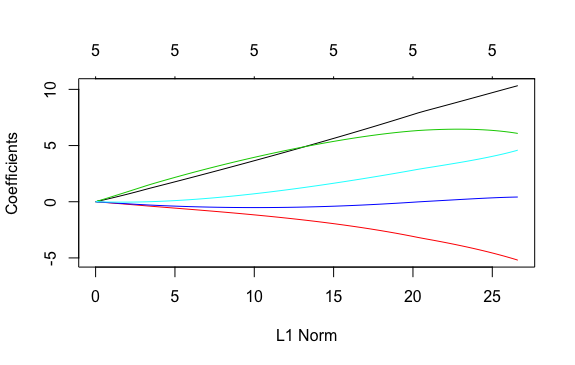
\includegraphics{fig/crime_ridge.png}}
\end{minipage}
\hspace{0.2cm}
\begin{minipage}{0.4\linewidth}
\scalebox{0.32}{\includegraphics{fig/crime_lasso.png}}
\end{minipage}
\caption{Koefficientstierne for ridge regression (venstre) og lasso (højre) plottet imod \(\ell_1\)-normen.} \label{fig:crime_koef}
\end{figure}
%
Variabel udvælgelsen for ridge regression og lasso illustreres på figur \ref{fig:LassoRig}.
%
\begin{figure}[H]
\centering
\begin{minipage}{0.4\linewidth}
\scalebox{0.7}{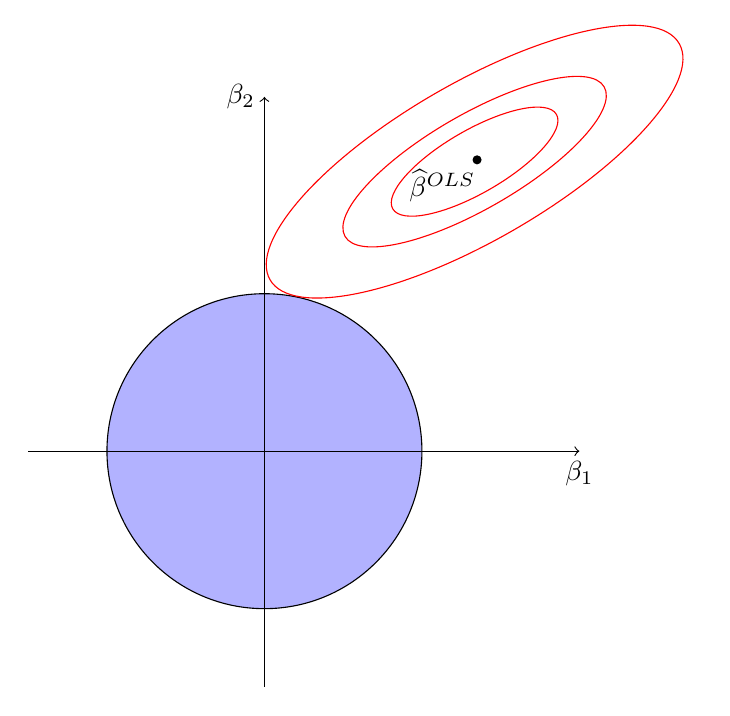
\begin{tikzpicture}
\draw [fill] (2.7,3.7) circle [radius=0.05];
\node [below left] (a) at (2.8,3.7) {$\widehat{\boldsymbol{\beta}}^\text{OLS}$};
\draw (0,0) circle (2cm) [fill= blue!30];
\draw [<-] (0,4.5) node [left] {$\beta_2$}-- (0,-3);
\draw[<-] (4,0) node [below] {$\beta_1$} -- (-3,0);
\begin{scope}[rotate = 30, red]
\clip[draw] (4.15,1.85) ellipse (3cm and 1cm);
\clip[draw] (4.15,1.85)ellipse (1.9 cm and 0.6 cm); 
\clip[draw] (4.15,1.85) ellipse (1.2 cm and 0.4 cm);
\end{scope}
\end{tikzpicture}}
\end{minipage}
\hspace{0.2cm}
\begin{minipage}{0.4\linewidth}
\scalebox{0.7}{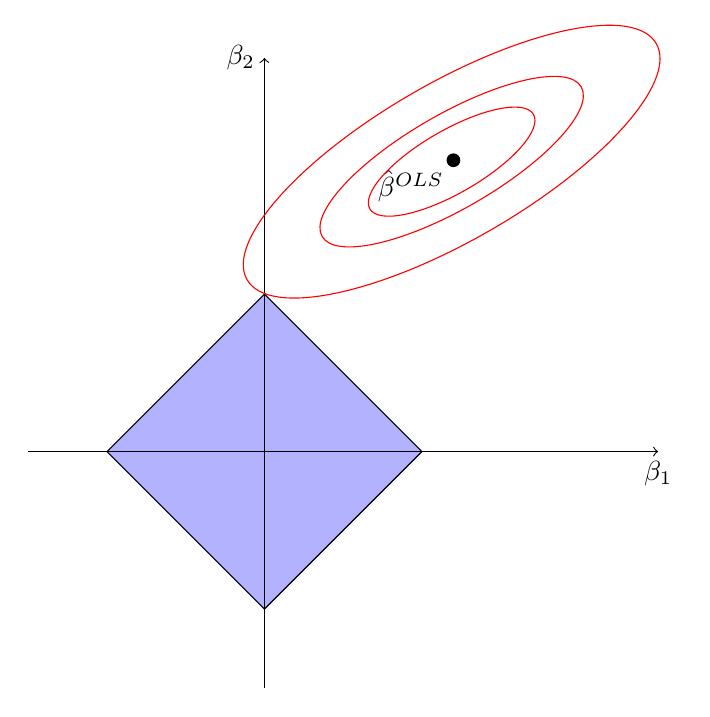
\begin{tikzpicture}
\draw [fill] (2.4,3.7) circle [radius=0.08];
\node [below left] (a) at (2.4,3.7) {$\hat{\beta}^\text{OLS}$};
\draw (-2,0) -- (0,2) -- (2,0)-- (0,-2) -- (-2,0)[fill = blue!30];
\draw [<-] (0,5) node [left] {$\beta_2$}-- (0,-3);
\draw[<-] (5,0) node [below] {$\beta_1$} -- (-3,0);
\begin{scope}[rotate = 30, red]
\clip[draw] (3.9,2) ellipse (3cm and 1cm);
\clip[draw] (3.9,2)ellipse (1.9 cm and 0.6 cm); 
\clip[draw] (3.9,2) ellipse (1.2 cm and 0.4 cm);
\end{scope}
\end{tikzpicture}}
\end{minipage}
\caption{Estimations illustration for ridge regression (venstre) og lasso (højre). 
De blå arealer er betingelsesområderne $\beta_1^2+\beta_2^2 \leq t^2$ og $\vert \beta_1 \vert+\vert \beta_2 \vert \leq t$, mens de røde ellipser er konturkurver for SSR. Konturkurverne har centrum i OLS estimatoren, $\hat{\beta}^\text{OLS}$.} \label{fig:LassoRig}
\end{figure}
%
For $p=2$ er betingelsesområdet for ridge regression givet ved $\beta_1^2 + \beta_2^2 \leq t^2$, og for lasso er det givet ved $\vert \beta_1 \vert + \vert \beta_2 \vert \leq t$.
Ellipserne omkring $\hat{\beta}^{\text{OLS}}$ er konturkurverne for SSR, dvs. SSR er konstant i en given ellipse. Værdien af SSR stiger, som ellipsen udvides fra $\hat{\beta}^{\text{OLS}}$.
Løsningen for ridge regression og lasso er givet ved det første punkt, hvor konturkurverne rammer betingelsesområderne.
Da ridge regression har et cirkulært betingelsesområde, vil skæringen med konturkurverne generelt ikke forekomme direkte på en akse.
Omvendt har lasso et regulært betingelsesområde med hjørner i hver akse, hvilket betyder, at hvis løsningen forekommer i et hjørne, da vil en af parametrene $\beta_j$ være lig 0.

Hvis $t$ er tilstrækkelig stor, da vil betingelsesområderne indeholde $\hat{\beta}^{\text{OLS}}$ og derfor vil ridge regression og lasso estimatorerne være lig OLS estimatoren.

På figur \ref{fig:LassoRig} har vi blot betragtet det simple tilfælde hvor $p=2$. 
Når \(p>2\) da vil betingelsesområdet for lasso være en polydron med mange hjørner, flade kanter og flader, som giver muligheder for at de estimerede parametre bliver lig 0.
%
\begin{lem}
Givet data \(\del{\y, \X}\), defineres et augmented datasæt
\begin{align*}
\mathbf{X}^* = \begin{bmatrix}
\mathbf{X} \\ \sqrt{\lambda} \mathbf{I}
\end{bmatrix}, \quad 
\mathbf{y}^* = \begin{bmatrix}
\mathbf{y} \\ \mathbf{0}
\end{bmatrix},
\end{align*}
hvor \(\X^* \in \mathbb{R}^{\del{n+p} \times p}\) og \(\y^* \in \mathbb{R}^{n+p}\). Da kan estimatoren for ridge regression udledes udfra mindste kvadraters metode.
\end{lem}
%
Beviset følger af simpel algebra og er derfor undladt.
%\begin{proof}
%Vi har, at
%\begin{align*}
%\del{\X^{*^T} \X^*}^{-1} \X^{*^T} \y^* &= \left( \begin{bmatrix}
%\mathbf{X} & \sqrt{\lambda} \mathbf{I}
%\end{bmatrix}
%\begin{bmatrix}
%\mathbf{X} \\ \sqrt{\lambda} \mathbf{I}
%\end{bmatrix} \right)^{-1}
%\begin{bmatrix}
%\mathbf{X} & \sqrt{\lambda} \mathbf{I}
%\end{bmatrix}
%\begin{bmatrix}
%\mathbf{y} \\ \mathbf{0}
%\end{bmatrix} \\
%&= \left( \mathbf{X}^T \mathbf{X} + \lambda \mathbf{I} \right)^{-1} \mathbf{X}^T \mathbf{y}.
%\end{align*}
%\end{proof}
%
\subsection{Udregning af lasso} \label{subsec:udregning_lasso}
Da lasso strafleddet ikke er differentialbel, findes der ikke en eksplicit løsning til optimeringsproblemet for lasso.
En simpel procedure kaldet \textit{coordinate descent} kan udfra Lagrange problemet udregne en numerisk løsning. 

\subsubsection{Single prædiktor: soft tresholding}
Vi betragter blot en enkelt prædiktor \(z_i\). 
Problemet, som vi skal løse, er da
\begin{align*}
\argmin_{\beta} \cbr{\frac{1}{2n} \sum_{i=1}^n \del{y_i - z_{i} \beta}^2 + \lambda \vert \beta \vert}.
\end{align*}
Som bekendt er standard proceduren at finde den første ordens afledede mht $\beta$, sætte denne lig 0 og isolere for $\beta$. 
Men vi bemærker, at \(\vert \beta \vert \) ikke er differentialbel i $\beta=0$.
Dette betegnes som en såkaldt \textit{subgradient}, hvilket vi vil beskrive nærmere i kapitel \ref{kap:optimeringsmetoder}.
Vi finder, at
\begin{align*}
\frac{\partial}{\partial \beta} \del{\frac{1}{2n} \sum_{i=1}^n \del{y_i - z_{i} \beta}^2 + \lambda \vert \beta \vert}
&= -\frac{1}{n} \sum_{i=1}^n \del{y_i - z_{i} \beta} z_i + \begin{cases}
-\lambda \quad &\beta < 0 \\
[-\lambda, \lambda] & \beta = 0 \\
\lambda & \beta >0 
\end{cases}  \\
&= -\frac{1}{n} \left\langle \mathbf{z}, \mathbf{y} \right\rangle + \beta + \begin{cases}
-\lambda \quad &\beta < 0 \\
[-\lambda, \lambda] & \beta = 0 \\
\lambda & \beta >0 
\end{cases},
\end{align*}
da $\frac{1}{n} \sum_{i=1}^n z_i^2=1$. Dette sættes lig 0 og vi isolerer $\beta$, hvoraf vi finder, at
\begin{align}
\hat{\beta} = \begin{cases}
\frac{1}{n} \left\langle \mathbf{z}, \mathbf{y} \right\rangle - \lambda, \quad &\frac{1}{n} \left\langle \mathbf{z}, \mathbf{y} \right\rangle > \lambda, \\
0 &\frac{1}{n} \left\langle \mathbf{z}, \mathbf{y} \right\rangle \leq \lambda, \\
\frac{1}{n} \left\langle \mathbf{z}, \mathbf{y} \right\rangle + \lambda, &\frac{1}{n} \left\langle \mathbf{z}, \mathbf{y} \right\rangle < -\lambda.
\end{cases} \label{eq:2.10}
\end{align}
Definer \textit{soft-threshold operatoren}
\begin{align*}
S_\lambda\del{x}=\text{sign}\del{x} \del{\vert x \vert - \lambda}_+,
\end{align*}
som trækker argumentet $x$ mod 0 med $\lambda$, og sætter den lig med 0 hvis $\vert x \vert \leq \lambda$. 
Figur \ref{fig:soft_thresholding_fct} illustrerer operatoren.
Da kan vi omskrive \eqref{eq:2.10} til
\begin{align*}
\hat{\beta} = S_\lambda \del{\frac{1}{n} \left\langle \mathbf{z}, \mathbf{y} \right\rangle}.
\end{align*}
%
\begin{figure}[H]
\centering
\scalebox{0.8}{\begin{tikzpicture}
\draw (-2.5,-2.5) -- (2.5,2.5);
\draw[dashed] (-2.5,-1.7) -- (-0.75,0) -- (0.75,0) -- (2.5,1.7); 
\draw[dotted] (2.5,1.7) -- (2.5,2.5);
%\draw node [label={[xshift=0.5cm, yshift=-0.8cm]$\del{0,0}$}] {};
\draw node [label={[xshift=2.75cm, yshift=1.8cm]$\lambda$}] {};
\draw [<-] (0,3) node [left] {$S_\lambda \del{x}$}-- (0,-3);
\draw[<-] (3,0) node [below] {$x$} -- (-3,0);
\end{tikzpicture}}
\caption[optional short text]{Soft thresholding funktionen $S_\lambda\del{x}=\text{sign}\del{x} \del{\vert x \vert - \lambda}_+$.} \label{fig:soft_thresholding_fct}
\end{figure}
%
\subsubsection{Multiple prædiktorer: cyclic coordinate descent}
Herefter kan vi betragte multivariate prædiktorer. 
%Gentagne cycle gennem prædiktorerne i en fast, men vilkårlig orden $j=1, 2, \ldots, p$, hvor koefficienten $\beta_j$ opdateres i det $j$'te step, ved at minimere objektfunktionen i dens koordinat, mens de resterende koefficienter $\cbr{\hat{\beta}_k, k \neq j}$ fastholdes deres nuværende værdier. 
Vi kan opskrive objektfunktionen i \eqref{eq:2.5} som
\begin{align*}
\frac{1}{2n} \sum_{i=1}^n \del{y_i - \sum_{k \neq j} x_{ik} \beta_k - x_{ij} \beta_j}^2 + \lambda \sum_{j = 1}^p \vert \beta_j \vert
\end{align*}
Definer den partialle residual $r_i^{(j)}=y_i - \sum_{k \neq j} x_{ik} \hat{\beta}_k$, som fjerner nuværende fit fra den $j$'te prædiktor.
Da er den j'te koefficient opdateret ved
\begin{align}
\hat{\beta}_j = S_\lambda \del{\frac{1}{n} \left\langle \mathbf{x}_j, \mathbf{r}^{(j)} \right\rangle}, \label{eq:2.14}
\end{align}
hvor \(r_i = y_i - \sum_{j = 1}^p x_{ij} \hat{\beta}_j \) er de fulde residualer.
Den beskrevne algoritme svarer til metoden \textit{cyclical coordinate descent}, som separat minimerer en konveks objektfunktion langs hver koordinat.
Under milde regularitetsbetingelser konvergerer løsningen til et global optimum.
Fra opdateringen \eqref{eq:2.14} ser vi, at algoritmen foretager en univariat regression af den partial residual på hver prædiktor, cycling gennem prædiktorerne indtil konvergens.

Hvis prædiktorerne er ortogonale, dvs $\frac{1}{n} \left\langle \mathbf{x}_j, \mathbf{x}_k \right\rangle = 0$ for alle $j \neq k$.
Da reduceres opdateringen \eqref{eq:2.14} til
\begin{align}
\hat{\beta}_j = S_\lambda \del{\frac{1}{n} \left\langle \mathbf{x}_j, \mathbf{y} \right\rangle}, \label{eq:ortogonal_lasso}
\end{align}
dermed er $\hat{\beta}_j$ blot soft-thresholded version af det univariate mindste kvadraters estimat af $\mathbf{y}$ regresseret imod $\mathbf{x}_j$. Således har vi en lukket løsning og ingen iterationer er påkrævet.

Ofte er vi interesseret i, at finde lasso løsningen for en mængde af \(\lambda\) værdier og ikke blot én fast lambda.
Metoden \textit{pathwise coordinate descent} kan anvendes hertil, ved at begynde med en værdi af \(\lambda\) som præcis er høj nok således at den optimale løsning er vektor bestående af \(0\).
Denne værdi er lig \(\lambda_{\max}=\max_j \left\vert \frac{1}{2} \left\langle \mathbf{x}_j, \y \right\rangle \right\vert\).
Da kan vi aftage \(\lambda\) med en lille mængde og køre coordinate descent undtil konvergens.
Aftage \(\lambda\) igen og anvende den tidligere løsning som en warm start, da kan vi kører coordinate descent indtil konvergens.
Hermed kan vi udregne løsningen over en grid af \(\lambda\) værdier. \\

Coordinate descent er særlig hurtig til at løse lasso problemet, da den koordinatvis minimizers er tilgængelig \eqref{eq:2.14}, og dermed er en iterativ søgning langs hver koordinat ikke nødvendig.
Derudover udnytter coordinat descent at lasso giver sparse løsninger.
For tilstrækkelige høje \(\lambda\) værdier er de fleste koefficienter lig $0$.

\textit{Homotopy metoder} er en alternativ teknisk til at løse lasso problemet. Disse producerer en helt sti af løsninger i en frekventiel sekvens, ved at starte med nul.
Denne sti er faktisk piecewise lineær.
Algoritmen kaldet \textit{least angle regression} (LARS) er en homotopy metode som effektivt konstruerer piecewise lineære stier.
En mere teoretisk gennemgang af coordinate descent og LARS algoritmen er givet i kapitel \ref{kap:optimeringsmetoder}.
%
\subsection{Frihedsgrader}
Antag vi har \(p\) prædiktorer og tilpasser en lineær regressions model udfra \(k\) af disse prædiktorer.
Hvis disse \(k\) prædiktorer vælges uafhængigt af responsvariablen, da "anvender" fitting proceduren \(k\) frihedsgrader.
Dette svarer til, at teststørrelsen for at teste hypotesen om at alle \(k\) koefficienter er 0, har en Chi-squared fordeling med \(k\) frihedsgrader.
%
Hvis valget af de \(k\) prædiktorer afhænger af responsvariablen, da forventes det at fitting proceduren anvender mere end \(k\) frihedsgrader. 
Sådan en fitting procedure kaldes \textit{adaptiv}, og tydeligvis er lasso et eksempel herpå.
Ligeledes er forward-stepwise proceduren adaptiv, hvor vi sekventiel tilføjer prædiktorer, som mindsker fejlen mest.
Her forventes det at modellen anvender mere end \(k\) frihedsgrader efter \(k\) step.
Derfor er antallet af frihedsgrader ikke nødvendigvis lig med antallet af ikke-nul koefficienter.
Men for lasso er antallet af frihedsgrader faktisk lig antallet af ikke-nul koefficienter, som vi nu vil beskrive.

Lad os først definerer hvad vi mener med frihedsgrader for en adaptiv fitted model. 
Antag at, vi har en additive-error model
\begin{align*}
y_i = f \del{x_i} + \epsilon_i, \quad i = 1, \ldots, n,
\end{align*}
hvor \(f\) er ukendt og \(\epsilon_i \sim iid \del{0, \sigma^2}\).
Lad \(\hat{\y}\) betegne \(n\) sample prædiktorer, da defineres 
\begin{align}
\text{df}\del{\hat{\y}} := \frac{1}{\sigma^2} \sum_{i=1}^n \text{Cov}\del{\hat{y}_i, y_i}. \label{eq:df_lasso}
\end{align}
Kovariansen tages her over det stokastiske i responsvariablen \(\cbr{y_i}_{i=1}^n\) hvor prædiktorerne fastholdes.
Antal frihedsgrader svarer da til indflydelsen hver respons mål har på dens prædiktion.
Desto bedre modellen tilpasser data, desto højere antal frihedsgrader.
Det kan vises, at for lasso med en fast strafparameter \(\lambda\) er antallet af ikke-nul koefficienter \(k_\lambda\) et unbiased estimat af frihedsgrader.

Som nævnt ovenfor anvender forward-stepwise regression mere end \(k\) frihedsgrader efter \(k\) step.
Lasso udvælger ikke blot prædiktorer, som bekendt øger antallet af frihedsgrader, men shrinks også koefficienterne mod 0 relativ til mindste kvadraters estimaterne.
Denne skrinkage er netop tilstrækkelig til at bringe antallet af frihedsgrader til \(k\).
Dette resultat er særligt nyttig, da det giver et kvalitativ mål af mængden af fitting som vi har opnået ved ethvert punkt på lasso stien.
Generelt er beviset for dette resultat meget besværligt.
Men i det ortogonale tilfælde ...

Ideen tages et skridt videre i sektion \ref{subsec:kovarians_test} hvor vi beskriver \textit{kovarians testen} til at teste significancen af prediktorerne ift lasso.
 
\subsection{Valg af tuning parameter og krydsvalidering}